\documentclass[UTF8, xcolor=table, fontset=adobe2]{beamer}
\usepackage[BoldFont,SlantFont]{xeCJK}
% \setCJKmainfont[BoldFont={Adobe Heiti Std},ItalicFont={Adobe Kaiti Std}]{AdobeSongStd-Light}
% \setCJKmainfont[BoldFont={Adobe Heiti Std},ItalicFont={Adobe Kaiti Std}]{SimSum} %Windows先编译使用这个字体

\usepackage{latexsym,amssymb,amsmath,amsbsy,amsopn,amstext,xcolor,multicol}
\usepackage{graphicx,wrapfig,fancybox}
\usepackage{pgf,pgfarrows,pgfnodes,pgfautomata,pgfheaps,pgfshade,pgfplots}
\usepackage{thubeamer}
\usepackage[backend=bibtex,sorting=none]{biblatex} % [参考文献格式](https://www.sharelatex.com/blog/2013/07/31/getting-started-with-biblatex.html) %mac IEEE not found
\usepackage{array}
\usepackage{bm}
\usepackage{caption}
\RequirePackage[font=footnotesize]{subcaption}
\usepackage{multirow}
\usepackage{booktabs}
\usepackage{tikz}
\usepackage{tikzscale}
\usepackage{animate}
\usepackage[normalem]{ulem}

\defbibheading{bibliography}[\bibname]{} %avoid printbibliography 自动生成目录
\addbibresource{../main.bib}
\setbeamertemplate{bibliography item}[text] 

\usepackage{boxedminipage} %for: bvh border
\def\fourgraphicswidth{0.35} %0.3\textwidth

\usepackage{algorithm} %%format of the algorithm
\usepackage{algpseudocode}
\floatname{algorithm}{算法}
\renewcommand{\algorithmicrequire}{\textbf{输入:}} % Use Input in the format of Algorithm
\renewcommand{\algorithmicensure}{\textbf{输出:}} % UseOutput in the format of Algorithm
\algrenewcommand{\algorithmiccomment}[1]{ $//$ #1}

\usepackage{listings}
\renewcommand\lstlistingname{代码}
\renewcommand\lstlistlistingname{代码}

\lstset{framexleftmargin=1.4em,
        xleftmargin=1.8em,
        basicstyle=\ttfamily\small,
        %frame=shadowbox, numberstyle=\tiny, breaklines=true,
        frame=single,
        numberstyle=\tiny, breaklines=true,
        keywordstyle=\color{blue!70}\bfseries,
        %commentstyle=\color{red!50!green!50!blue!50},
        rulesepcolor=\color{red!20!green!20!blue!20},
        numbers=none,fontadjust=true}
\lstdefinelanguage{shader}{morekeywords={uniform, layout, uniform, vec2, vec3, vec4, in, out, gl_Position, dot, flat, int ,float, gl_VertexID, xyz, w, x, y, z, location, version, sampler2DRect, bgr, gl_FragData, texture2DRect, gl_TexCoord,for,xy},morecomment=[l]{//}}

\begin{document}

\setbeamerfont{footnote}{size=\tiny}
\setbeamerfont{caption}{size=\scriptsize}
\setbeamertemplate{caption}[numbered]
\setbeamerfont{subsection in toc}{size=\footnotesize}
\renewcommand*{\bibfont}{\footnotesize}

\graphicspath{{../}}

\title[基于RDMA的分布式内存存储数据传输优化]{基于RDMA的分布式内存存储\\数据传输优化}
\author[兰靖]{(申请中山大学工学学士学位论文答辩报告)\\ \vskip 20pt 学~~~生:兰~~靖}
\institute[中山大学~计算机学院~\&~计算机科学与技术]{\small \vskip 27pt 计算机学院~计算机科学与技术}
\date{\small \vskip -30pt 二〇二二年五月}

%% make title %%
\frame{
        \titlepage
        \vspace{-25mm}
}

% \subsection*{目录}
% \frame {
%         \frametitle{目录}
%         \tableofcontents[sections={<1-7>}]
% }

%%
% 引言或背景
% 引言是论文正文的开端,应包括毕业论文选题的背景、目的和意义;对国内外研究现状和相关领域中已有的研究成果的简要评述;介绍本项研究工作研究设想、研究方法或实验设计、理论依据或实验基础;涉及范围和预期结果等。要求言简意赅,注意不要与摘要雷同或成为摘要的注解。
% modifier: 黄俊杰(huangjj27, 349373001dc@gmail.com)
% update date: 2017-04-15
%%

\chapter{绪论}
% 定义,过去的研究和现在的研究,意义
\label{cha:introduction}
\section{选题背景与意义}
\label{sec:background}
% What is the problem
% why is it interesting and important
% Why is it hards, why do naive approaches fails
% why hasn't it been solved before
% what are the key components of my approach and results, also include any specific limitations,do not repeat the abstract
%contribution
% 引言是论文正文的开端,应包括毕业论文选题的背景、目的和意义;对国内外研究现状和相关领域中已有的研究成果的简要评述;介绍本项研究工作研究设想、研究方法或实验设计、理论依据或实验基础;涉及范围和预期结果等。要求言简意赅,注意不要与摘要雷同或成为摘要的注解。

分布式计算框架是一种复杂的平台软件。传统的并行计算范式如信息传递接口(MPI)和分区全局地址空间(PGAS),通常为编程者提供丰富的调用接口和灵活的编程空间。
然而,使用这些编程标准的门槛过高:编程者通常需要自己管理多台机器的状态,特别是内存的分配和使用;编程者还需要使用给定的标准原语,精确地规定多个进程之间的通信和协作方式,
这通常需要大量时间和精力;另外使用这些范式将导致程序和功能的强耦合——编程者很可能不得不重新编写代码来更新程序的逻辑。因此,现代分布式计算框架通常承担了上述硬件管理的角色,
并针对目标任务类型,为用户设计尽可能少、但简单易用的功能接口,来降低集群的使用难度。传统的分布式计算框架,例如Mapreduce和Spark,都是面向大规模数据分析而设计的。然而,近些年
以强化学习、复杂工作流等为代表的复杂计算需求,需要更灵活的框架支持。加州大学伯克利分校RISELab实验室提出的Ray和芝加哥大学Globus实验室提出的Parsl是其中两个典型。这些框架
吸取了云计算领域“函数即服务(Function as a Service, FaaS)”的设计思想,能够细粒度地以函数为单位将任务调度到集群上执行,同时依然对用户隐藏绝大部分实现细节。Ray通过分布式内存对象存储Plasma,
实现了框架完全自主的集群内存管理,使用户可以专注于实现功能逻辑。Ray在保持易用性的前提下,极大地提升了计算框架的灵活性,用户只需要修改几行代码就能将单进程程序扩展到整个集群。

高性能集群、或超算集群,是一种以高端处理器、计算卡、高性能网络、大容量存储为核心硬件的计算集群。随着大数据应用的丰富、超大规模人工智能模型的出现,高性能集群和超级计算机正在变得愈发重要。
首先,高性能计算机拥有普通机器不能比拟的计算能力,主要表现为高端的多核处理器和计算卡。而随着大模型时代的到来,应用对集群网络的需求逐渐提高,高性能网络所表现出的高带宽、低延迟等特性
也逐渐受到了更多的关注。在超算集群中,网络性能上的优势很大程度上来自于对远程直接内存访问(RDMA)机制的支持。然而,要利用RDMA,用户必须在应用中实现基于RDMA的通信机制,而不能依赖于操作系统内核提供的系统调用。
因此大多数基于套接字(Socket)的网络应用都不能在高性能集群中获得显著的性能提升。分布式计算框架Ray并不例外,其分布式内存存储Plasma目前仅有对传统TCP/IP协议的支持,因而在超算集群上无法发挥出应有的网络性能,从而进一步影响Ray的总体性能。

当前,超算集群普遍使用的是英伟达(Nvidia)公司的Infiniband高速网络。对于使用Socket通信的网络程序,该架构通过“基于Infiniband的互联网协议(IPoIB)”实现支持。值得注意的是,这是一种非原生支持,
已经有多个工作表明,其网络性能和直接使用RDMA技术相比具有明显差距。因此,本研究的目的即:我们是否能为分布式内存存储Plasma,提出并实现一种支持RDMA机制的内存通信协议,从而让Plasma乃至整个Ray框架在
现代超算集群上获得更好的性能?从超算研究的趋势来说,应用软件和先进超算硬件之间的隔阂,正在逐渐成为大家关注的热点。随着超级计算机和云计算两个领域的融合,会有越来越多的软件运行在高性能集群中。
而它们通常没有针对高性能硬件提供支持——通过提供软件对高性能硬件的支持,我们能够将相当多应用的性能提升到全新的水平。

\section{国内外研究现状和相关工作}
\label{sec:related_work}

\subsection{远程直接内存访问技术(RDMA)}



\subsection{基于RDMA技术的内存系统}

\subsubsection{高并发内存系统}

\subsubsection{分布式内存系统}

\section{论文主要研究内容}

本工作研究的是为分布式内存存储Plasma,提供一种原生支持RDMA技术的通信机制,从而使其在现代超算集群上获得更优的数据传输性能。

这一工作存在以下挑战:

\begin{enumerate}
	\item 目前RDMA编程仍然是极为“小众”的技术,如何能基于有限的资料和研究实现高性能的网络通信机制。
	\item 如何在尽可能不破坏项目整体结构的情况下,为Plasma提供原生RDMA通信机制。这要求优化后的程序可以无缝实现两种机制的兼容。
	\item 针对Ray框架中可能出现的大小不一的数据,如何实现该机制使得Plasma能够在尽可能多的范围内都能获得最优的网络性能。
\end{enumerate}

\section{论文结构与章节安排}
\label{sec:arrangement}

本文的剩余章节共分为五章,这些章节的内容安排如下:

第二章为本科生毕业论文写作与印制规范。本章节就学校的规范,逐点进行描述,并给出来了相关例子说明本模板在格式上的正确性。

第三章为本模板的使用说明。

第四章为可用的\LaTeX 的代码段方便大家进行编辑。

第五、六章是本文的最后两章,作为空白章节例子。


\chapter{Plasma分布式内存存储架构和性能分析}

\section{Plasma架构分析}

Plasma分布式存储架构由多个进程组成。通过将控制面、数据面上的任务解耦到不同的进程,我们可以较为方便地对其软件架构进行改进。
\autoref{fig:plasma_arch}展示了Plasma集群的组织结构。

\begin{figure}[h] 
    \centering
    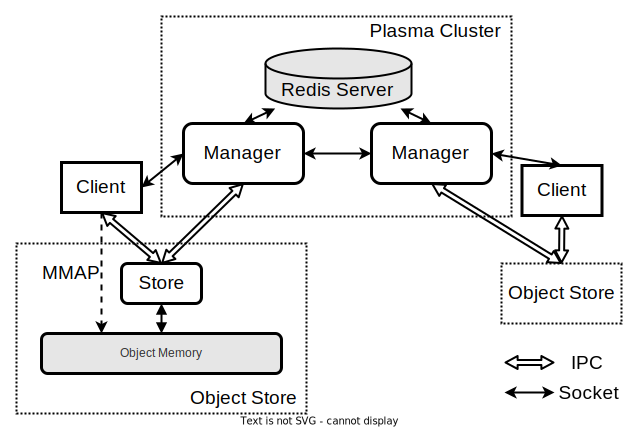
\includegraphics[width=0.75\textwidth]{image/chap02/plasma_arch.png}
    \caption{Plasma存储架构}
    \label{fig:plasma_arch}
\end{figure}

\subsection{Plasma对象存储架构}

对象存储(Object Store)是Plasma运行的最小单元,即Plasma在任意单节点上运行时,可以不需要连接到管理进程(Manager)和Redis数据库。
\autoref{fig:plasma_arch}中左下方部分展示了这一架构。对象存储的基本架构遵循用户端-服务端的特征。Store进程负责直接操作和管理机器内存。
当用户(Client)进程发起创建对象请求时,会将关键元数据——即对象编号(id)、元数据大小、数据大小等通过进程间通信(IPC)发送给Store进程。
值得注意的是,Plasma使用Unix域套接字(Unix Domain Socket)作为进程间通信方式,这一方式允许用户端以类似套接字的方式,通过操作系统内核与本机内的另一个进程交换数据。

Plasma利用MMAP映射机制对内存对象操作进行了性能优化。当前常见的内存数据库如Redis,用户端进程和服务端需要直接交换数据以完成创建、读取等操作。而Plasma利用了MMAP机制,
使得客户端与服务端能够共享内存空间:

\begin{enumerate}
    \item 创建对象时,服务端使用MMAP映射分配内存空间,将其与一临时文件映射。
    \item 服务端通过IPC,将上述临时文件的文件描述符(file descriptor,fd)传递给用户进程。
    \item 用户进程使用相同的文件描述符fd再次调用MMAP。
\end{enumerate}

如此,MMAP向Store进程和用户进程返回同一个内存地址,用户进程能够直接读取、操作数据库中的内存对象。这一架构能够将数据库读取操作的开销
优化到$O(1)$时间复杂度,使Plasma针对大型对象仍然具有优秀的吞吐能力。Plasma在对象存储架构中定义了如下操作原语:

\begin{table}[h]
    \centering
    \caption{Plasma客户端接口}
    \begin{tabular}{*{2}{c}}
        \toprule
        接口定义 & 接口描述      \\
        \midrule
        plasma\_contain(id)                                    & 查询对象是否存在   \\
        buf $\leftarrow$ plasma\_create(id, fields, values)    & 创建参数/数据为fields/values的对象   \\
        plasma\_seal(id)                                       & 封装对象使其对其他进程可见   \\
        plasma\_release(id)                                    & 释放对象,引用计数减一(为0则删除)   \\
        buf $\leftarrow$ plasma\_get(id, fields)               & 读取对象   \\
        plasma\_delete(id)                                     & 删除对象   \\
        \midrule
        plasma\_connect(store\_addr, manager\_addr)            & 连接到Store和Manager \\
        plasma\_subscribe(id)                                  & 等待一个对象在本机被创建 \\ 
        \bottomrule
    \end{tabular}
    \label{tab:store_api}
\end{table}

\subsection{Plasma集群架构}

Plasma存储将其集群架构单独实现为Manager进程,多个进程以及一个Redis数据库共同构成其集群架构,\autoref{fig:plasma_arch}中上方
展示了将Plasma连接成集群的架构。Plasma在集群架构中定义了如下操作原语:

\begin{table}[h]
    \centering
    \caption{Plasma集群接口}
    \begin{tabular}{*{2}{c}}
        \toprule
        接口定义 & 接口描述      \\
        \midrule
        buflist $\leftarrow$ plasma\_fetch(ids)               & 将id列表中的对象拉取到本地存储   \\
        \bottomrule
    \end{tabular}
    \label{tab:manager_api}
\end{table}

管理者(Manager)进程仅处理用户进程发出的一种请求,即输入一个id列表,执行一次拉取(fetch)操作:

\begin{enumerate}
    \item Manager对列表中的每个id,从集群中查找对应数据对象的位置。 
    \item 本地Manager与存有这一对象的另一个Manager建立连接,拉取数据。
    \item Manager和Store交互将数据保存到本地——对Store进程来说,Manager只是普通的Client进程。
\end{enumerate}

在这一过程中,Plasma依赖于Redis提供的数据库服务。每当Client进程创建并封装数据对象时,它将借助Manager与Redis服务器建立通信,并更新该对象在集群中的分布。
因此Manager在拉取数据的过程中(上述步骤2),必须先从Redis得到数据分布,才能开始一次数据传输。

\section{基于套接字的Plasma通信机制}

Plasma实现了基于套接字(Socket)的数据传输机制。通过访问Redis服务器获得对象处在的目标节点后,Manager会逐一尝试建立Socket连接,并拉取数据。
其通信机制如\autoref{fig:sock_protocol}所示:

\begin{figure}[h] 
    \centering
    \includegraphics[width=0.75\textwidth]{image/chap02/sock_protocol.png}
    \caption{基于套接字的Plasma通信机制}
    \label{fig:sock_protocol}
\end{figure}

发起者(Receiver)首先将一条类别为PLASMA\_TRANSFER的消息发送给存有数据对象的Manager进程。在得知需要发送的对象id后,发送方通过向Store调用查询操作获得了
数据的缓冲区地址。需要注意的是Plasma的读取操作具有常数的时间复杂度,因而会马上返回。发送方(Sender)会将查询到的元数据(主要是数据大小)通过PLASMA\_DATA消息返回给接收方,接收方便会
向Store创建一个同id的对象,获得分配的内存空间。最后双方分别进入发送/接收函数,分批将数据转移到本地缓冲区中。

在Plasma实现中,默认一次发送4kb大小的数据。

\section{Plasma存储和传输性能分析}

为了分析Plasma存储运行在超算上可能存在的性能瓶颈,我们在天河高性能集群上对Redis和Plasma进行了存储和传输上的性能测试。

\subsection{存储性能测试}

\subsection{数据传输测试}
\chapter{基于RDMA的Plasma数据传输机制实现}
\label{cha:implementation}

在本章节中,我们将基于上一章对Plasma架构和性能的分析,提出并实现一种适应各大小数据的高吞吐数据传输机制。由于跨节点通信完全由Manager进程完成,因此在本章节中,
如无特殊说明,进程均指的是Manager进程。

\section{连接的建立和复用}
\label{sec:ib_con}

要进行双边(Send/Recv)和单边(Read/Write)通信,通信两端都需要首先为建立Infiniband连接。和套接字简单的连接过程不同,在双方能够通过发送事务传送数据之前,首先要完成
如下准备工作:

\begin{enumerate}
	\item 创建IB上下文(Context);得到机器的IB设备列表,并打开其中一个设备(网卡)。用户可以在此时读取网卡的部分硬件参数。
	\item 创建一个保护域(Protection Domain,PD)。这是一种管理机制,后续创建的数据结构只有处在同一个保护域中才能相互访问。
	\item 创建发送/接收缓冲区,并将其注册为内存区域(Memory Region,MR)。这一操作的主要目的是使内存页面驻留在物理内存中,防止操作系统通过换页等机制
	将内存空间移出。由于RDMA实现在用户态,缓冲区的检查和数据收发都需要由用户正确地管理——否则会导致旧数据被覆盖等错误。
	\item 创建完成队列(Completion Queue,CQ)。在双边通信中,用户通过拉取完成队列来检查通信事务的执行结果。
	\item 双方进程创建并连接队列对(Queue Pair,QP)。使用可靠连接(RC)服务时,一对队列对在建立连接后只能相互发送数据。要建立一对连接,
	用户需要使用套接字等基础通信手段交换队列对的关键参数:网卡设备的本地编号(lid)和队列对编号(qp\_num)。
\end{enumerate}

IB连接的建立流程有显著的时间开销。在实验中,我们通过测试发现这一流程将引入额外300ms左右的延迟开销。这一结果和Frey等\cite{frey2009minimizing}的描述基本一致。尽管由于面向单机,这一开销
在高并发内存系统的相关研究中并没有得到很大重视,然而这对于分布式内存系统Plasma来说是重要的。后者在每个节点都要部署进程,其IB连接以$O(N^2)$速度扩大规模。
加之Plasma具有不规律的通信特征,即便是基于套接字的实现,大量并发的连接请求也造成了显著的性能损失。因此在集群中反复建立IB连接更是难以忍受的。

所以,我们必须在节点间复用IB连接。值得注意的是,步骤3创建并固定内存缓冲区占用了上述过程的主要时间开销,并且这一过程不依赖于队列对的连接。所以,在IB优化的Plasma
实现中,我们先尝试建立队列对,\textbf{最后}才分配缓冲区。我们为每个进程维护了一个以网卡编号lid为键的哈希表。哈希表中的每个元素,以一个数据结构保存着一对IB连接的必要数据。因此,当两个进程尝试建立连接时,
它们将首先通过套接字交换lid,并查找哈希表。如果两个节点曾经建立过IB连接,那么双方将复用第一次分配好的缓冲区。通过这一改进,Plasma仅有初次IB连接会感受到明显的传输延迟,而再次建立连接的时间开销大幅降低。

\section{基于双边通信的传输协议}
\label{sec:send}

针对内存数据库常见的较小数据,我们提出了基于双边通信机制的传输协议。这一机制的优势在于,能够充分利用两节点间\textbf{预先分配}的发送/接收缓冲区。其示意图如\autoref{fig:send_protocol}所示:

\begin{figure}[h]
	\centering
	\includegraphics[width=0.7\textwidth]{image/chap03/send_protocol.png}
	\caption{基于双边通信的传输协议}
	\label{fig:send_protocol}
\end{figure}

\textbf{双边协议的实现:}在该传输协议中,通信双方(Sender/Receiver)在握手发生前必须首先通过一次post\_recv操作将一个接收事务放入到接收队列中。这是因为任何一个发送事务在完成时,连接的接收队列必须有可用的接收事务对应,
否则通信无法发生。在本实现中,由于每个进程都维护着与其他进程的IB连接和对应的缓冲区,因此做法是在连接建立时,进程都首先将一个接收事务放入到和该连接关联的接收队列中。这样我们就能确保第一次数据传输的
握手发生前,接收队列总是存在可用的接收事务。

当数据发送方收到类型为PLASMA\_TRANSFER的消息后,和套接字协议一样,它首先调用plasma\_get函数得到了数据缓冲区的地址。然后,发送方将对象id、数据大小等关键元数据通过PLASMA\_DATA消息传递给数据接收方。
之后,发送方将数据从得到的内存拷贝到预留的发送缓冲区,调用post\_send将数据通过RDMA发送到接收方预留的接收缓冲区。值得注意的是:

\begin{enumerate}
	\item 以此协议发送和接收数据,发送方和接收方在这一阶段都会产生一次用户态的内存拷贝。如\autoref{fig:send_protocol}中虚线箭头所示:为了复用预先分配的内存缓冲区、避免重复的内存分配和注册,
	发送前数据必须要拷贝到固定缓冲区,接收时必须要从固定缓冲区拷贝。在较小数据的传输中,这两次内存拷贝的开销占比较低,因而是较优的通信方案。
	\item RDMA传输的数据和接收方调用plasma\_create的顺序是不定的,但不影响该协议的正确性,\autoref{fig:send_protocol}展示了其中一种顺序。数据可能先于元数据到达,也可能后于元数据到达。但不论事件以何种顺序发生,
	接收方都会在元数据到达后,调用plasma\_create创建对象,然后轮询完成队列(CQ),确保对象数据已经到达。最后,接收方通过一次用户态的内存拷贝,将数据存到指定位置。在这里,轮询完成队列是一种同步机制——如果数据已经到达,
	它将立刻返回;否则将阻塞,直到数据在缓冲区准备就绪。这一现象展示了RDMA通信的异步性。
\end{enumerate}

\textbf{接受事务的补充}:数据到达后,由于接收事务被消耗了,接收方在取出数据、确认缓冲区可覆盖之后,需要重新提交一个接受事务等待下次使用。
在这一步,我们希望从完成队列里面获取接收数据的内存地址,以便将一个指向相同地址的接收事务补充到接收队列中。这一目的可以通过事务编号(Work Request ID)完成:IB Verbs的事务编号是一个64位无符号整数,因此我们可以直接将接收地址
作为事务的编号——这样还很方便地解决了事务编号的唯一性。

\textbf{发送确认信息:}和基于套接字的协议不同,此时接收方还需要发送一个确认(ACK)消息给发送方。这同样是一个同步机制。因为发送方并不知道接收方何时重新准备好了
接收事务和缓冲区(而这在套接字编程中是无需担心的),这一ACK消息用于启动下一轮的数据发送。如果没有这一确认消息,发送方可能会在接收方还没有配对的接收事务时再次发送,进而导致程序错误。

\section{基于单边通信的传输协议}
\label{sec:read}

\textbf{双边协议的局限性:}在实现了上述基于双边通信的传输协议后,在实验中我们已经观察到了相当的吞吐提升——即便完成传输所需的通信次数相比套接字协议可能更多,但RDMA通信的延迟极低。
然而,进一步对程序在较大数据的传输测试中进行性能采集,我们发现当数据规模增加时,程序将大量CPU时间用于用户态的数据拷贝(即memcpy调用)。
虽然,用户态的内存拷贝性能相当可观,在数据较小时产生的额外延迟并不显著,但随着数据增长到1MB大小,CPU的处理能力无法跟上RDMA网卡的吞吐能力,成为了性能瓶颈。

对于上述双边通信的传输协议,选择用数据拷贝代替反复创建/销毁缓冲区是出于对后者较大开销的忌惮。这一前提在大型数据下是否还成立呢?结论是否定的,在第四章的实验和分析中,我们确认了内存空间分配+注册具有更好的扩展性:在数据较大时,
反而是CPU直接复制同样大小的数据更耗费时间。这一观察驱使我们进一步为较大数据单独设计一个支持零拷贝的传输协议。我们实现了基于单边读(One-sided Read)的约会(Rendezvous)协议,其示意图如\autoref{fig:read_protocol}所示:

\begin{figure}[h]
	\centering
	\includegraphics[width=0.7\textwidth]{image/chap03/read_protocol.png}
	\caption{基于单边通信的传输协议}
	\label{fig:read_protocol}
\end{figure}

\textbf{单边协议的实现:}在基于单边读的传输协议中,使用了与传统通信原语极为不同的读语义:发送方不再事实上承担发送数据的任务,而是由接收方直接从远端内存拉取数据到本地。在接受到PLASMA\_TRANSFER消息,且通过plasma\_get函数调用获得了数据对象的地址后,
发送方直接向RDMA网卡注册MMAP映射返回的内存空间。因此,内存数据将在原地被网卡读取并发送,而不再依靠预先分配的固定缓冲区。接下来,接收方将会收到发送方传递的元数据、创建内存空间,并同样向RDMA网卡注册plasma\_create返回的内存地址。
需要注意的是,这一阶段发送方需要额外地将本地内存地址(raddr, rkey)发送到接收方处,才能正确地引导后者拉取内存数据。
此时,双方的内存空间都已原地(in-place)成为可用的发送/接收缓冲区,接收方发出一个单边读请求,就能完成对象的复制。最后,接收方通过一个结束(FIN)消息通知对方注销缓冲区,也同时注销自己的缓冲区。一次数据传输就完成了。

\textbf{单边协议的技术优势:}在这一协议中,我们将内存数据所处空间原地注册为缓冲区,这一协议具有一些优势:传输仅需要两个来回(一次握手和一次传输),相比之下双边协议的来回数依赖于固定缓冲区的大小;实现比前者更简单;为发送方和接收方各节省了一次用户态的数据拷贝,
实验表明这一特性在数据较大时具有明显性能优势。

\section{传输机制的完整实现}

\textbf{两种传输机制的混合实现:}上述的两种传输协议具有不同的性能表现,本质上是在两种固定开销中进行权衡:双边传输协议使双方增加了一次内存拷贝,避免了重复的内存注册/注销操作;单边传输协议每次传输都需要注册/注销内存,但真正实现了(用户态/内核态)内存零拷贝。直观上来说,
前者适合发送小数据,而大型数据则应该采用后者传输。幸运的是,通过确定一个分界点,我们能将两种机制混合实现,而只需要对Plasma主逻辑做出微小改动。定义常量IB\_READ\_MIN\_SIZE为采用单边协议的最小数据量,就能在函数调用前确定使用的协议。
下方\autoref{server}展示了Plasma发送端的处理逻辑:

\begin{algorithm}[H]
	\caption{服务端发送机制}\label{server}
	\KwIn{连接上下文$conn$,对象标识符$id$}
	$buf$:缓冲区,$S_d$:数据大小,$S_m$:元数据大小 \\
	读取对象内存区域:$buf, S_d, S_m \leftarrow$ plasma\_get($id$) \\
	发送元数据:send\_message($conn, S_d, S_m, id$) \\
	\eIf{$S_d$ + $S_m$ $\leq$ IB\_READ\_MIN\_SIZE}{
		发送本地地址:ib\_send\_read\_info($conn, buf$) \\
		等待单边读:ib\_wait\_object($conn, buf$)
	}{
		双边发送协议:ib\_send\_object\_chunk($conn, buf$)
	}
	释放对象:plasma\_release($id$)
\end{algorithm}

和发送方不同,接收方需要在收到对象元数据后在本地存储中创建该对象;并且,在通过RDMA接收数据并复制到合适位置后,还需要封存对象,使得对象能对集群中的其他进程可见。
下方\autoref{client}展示了Plasma接收端的处理逻辑:

\begin{algorithm}[H]
	\caption{客户端接收机制}\label{client}
	\KwIn{连接上下文$conn$}
	$buf$:缓冲区,$S_d$:数据,$S_m$:元数据大小,$id$:对象标识符 \\
	接收元数据:$S_d, S_m, id \leftarrow$ recv\_message($conn$) \\
	创建对象内存区域:$buf \leftarrow$ plasma\_create($id, S_d, S_m$) \\
	\eIf{$S_d$ + $S_m$ $\leq$ IB\_READ\_MIN\_SIZE}{
		$raddr$:远端内存地址 \\
		接收远程地址:$raddr \leftarrow$ ib\_recv\_read\_info($conn$) \\
		单边读协议:ib\_read\_object($conn, buf, raddr$)
	}{
		双边接收协议:ib\_recv\_object\_chunk($conn, buf$)
	}
	确认对象:plasma\_seal($id$) \\
	释放对象:plasma\_release($id$) \\
\end{algorithm}

因此,优化后的Plasma程序能够在运行时通过判断拉取的数据大小来调整传输协议。那么,为了在不同的数据大小上都获得最优的传输性能,我们需要通过实验
获得IB\_READ\_MIN\_SIZE的最优取值。在之后的实验中,我们将对套接字协议、双边传输协议和单边传输协议分别进行详细的性能测试,从而确定出最优的参数,
得到最优的总体性能。

\textbf{IB连接的完整实现:}下方\autoref{lst:label}展示了支持混合传输机制的最终实现。
每当两个进程之间按照\autoref{sec:ib_con}所描述的流程建立一个IB连接时,它们将分别创建该数据结构的一个副本,并将其插入到哈希表中。之后,它们通过维护
这个结构来完成双边或单边通信。

\begin{minipage}{\linewidth}	
\begin{lstlisting}[style=sysucpp, label={lst:label}]
typedef struct {
  struct ibv_qp *qp;
  struct ibv_wc *wc;
  struct ibv_cq *cq;
  struct ibv_mr *recv_mr;
  struct ibv_mr *send_mr;
  struct ibv_mr *read_mr;
  uint8_t *ib_recv_buf; // send/recv buffers are pre-pinned
  uint8_t *ib_send_buf;
  uint8_t *ib_read_buf; // read buffer is pinned and registered on-the-fly
  int64_t bufsize;

  uint32_t rkey;
  uint64_t raddr;

  // key and handle to construct a hash table
  int slid;
  UT_hash_handle hh;
} IB_pair_info;
\end{lstlisting}
\end{minipage}

在该结构中,qp为IB连接中本地的队列对结构,Verbs通过它来确定消息的目的地;cq为完成队列,进程以此检查事务的完成情况;wc则为存放完成队列项(CQE)的缓冲区——进程每次轮询完成队列cq后,获得的元素都将暂存在这里等待检查。

此外,每个进程还要分别维护三个内存缓冲区buf和它们关联的内存空间(MR)。其中发送缓冲区和接收缓冲区如\autoref{sec:send}所述,在连接建立时就将预先创建好,等待数据的发送/接收。
而读缓冲区在此时则被赋值为空(NULL),只有在单边读协议发生时,该缓冲区才被即时(on-the-fly)分配、关联的内存空间同时被注册。如\autoref{sec:read}描述,进程在单边读之前需要获得
对方读缓冲区的索引和内存地址,我们同样在结构体中为这些变量分配了位置。
\chapter{性能测试与结果分析}

\section{实验环境配置}

本段将简单介绍运行Plasma的必要环境配置。这包括进行性能测试的集群硬件配置,以及编译、运行Plasma所需的其他软件要求。

\subsection{天河高性能集群硬件简介}

运行测试的天河高性能集群有超过100台CPU服务器,并由100GB的Infiniband高速网络连接而成。每个CPU节点的关键配置如下所示:

\begin{table}[h]
    \centering
    \caption{天河CPU服务器硬件配置}
    \begin{tabular}{*{4}{c}}
        \toprule
        硬件组件  & 数量 & 硬件型号 & 参数配置 \\
        \midrule
        CPU  	 & 2  & Intel(R) Xeon(R) Gold 6150 & \makecell{18核 @2.7GHz \\ L1 Cache 64K \\ L2 Cache 1024K \\ L3 Cache 25344K} \\
        \midrule
        内存 	 & 12 & / & \makecell{16Gb DDR4 \\ with ECC} \\
        \midrule
    	以太网卡 & 1  & Mellanox MT27710 Family [ConnectX-4 Lx]   & 25Gb/s \\
    	IB网卡   & 1  & Mellanox MT27700 Family [ConnectX-4] & 100Gb/s \\
        \bottomrule
    \end{tabular}
    \label{tab:hardware_config}
\end{table}

每个CPU服务器配备有双路Intel至强金牌处理器。每个CPU为6通道16G内存,因此每节点内存总量为192Gb。两路处理器形成两个NUMA节点,每节点上分别挂载有一张网卡。
该型服务器的硬件拓扑图如\autoref{fig:server_block}所示:

\begin{figure}[h]
	\centering
	\includegraphics[width=0.7\textwidth]{image/chap04/server_block.png}
	\caption{天河CPU服务器硬件拓扑}
	\label{fig:server_block}
\end{figure}

需要注意的是,以太网卡和IB网卡分别挂在两个CPU的PCI-E Switch上,因而IB网卡只有在访问本NUMA节点的一半内存时拥有最佳性能——而访问远离它的CPU所控制的一半内存将会有
较大的性能损耗(\autoref{fig:server_block}中\textbf{红色访存路线})。这一特性对基于RDMA的网络通信性能有明显的影响,因此在实验中需要相应调整运行配置。

\subsection{软件环境简介}

\autoref{tab:software_config}展示了本章节各性能测试所运行的软件环境。操作系统一栏展示了天河高性能集群使用的Linux操作系统版本;软件依赖指的是成功编译出可正常执行
的Plasma程序所需要的前置软件;测试软件则表示为了编译基准测试程序、运行测试程序所需要的前置软件。软件名后的数字串分别表示这些软件的版本。

\begin{table}[h]
    \centering
    \caption{天河CPU服务器软件环境}
    \begin{tabular}{*{3}{c}}
        \toprule
        软件类型 & 软件名称  & 作用描述 \\
        \midrule
        操作系统 & CentOS Linux 7 & Linux内核版本3.10.0-957.el7.x86\_64 \\
        \midrule
        \multirow{3}{*}{软件依赖} & Redis@3.2.3 & \makecell{Redis服务器存放对象在Plasma集群的分布 \\ ae事件循环库驱动Plasma进程} \\
    	 & \makecell{uthash \\ utlist \\ utarray \\ utstring}@2.0.1 & \makecell{基于宏的C语言头文件库,\\ 包装了哈希表等高级数据结构} \\
		 & gcc@9.3.0 & 编译Redis和Plasma \\
        \midrule
    	\multirow{2}{*}{测试软件} & openmpi@4.1.1 & 编译基于MPI的多节点性能测试 \\
    	 & numactl@2.0.14 & 控制MPI进程在NUMA架构下的绑核运行 \\
        \bottomrule
    \end{tabular}
    \label{tab:software_config}
\end{table}

\section{NUMA架构对存储性能的影响}

\section{协议性能测试}

\section{结果分析}
\chapter{总结与展望}

\section{本研究工作总结}

在本文的研究中,我们探索了一种在最新的分布式计算框架和现代高性能硬件之间进行适配的性能优化。Plasma作为支撑分布式计算框架Ray的分布式内存管理组件,
在设计上并没有考虑过超算集群独特的硬件特性,特别是支持RDMA通信机制的高速网络,因而无法在超算集群上得到最佳的传输性能。我们首先通过跨节点的性能测试
验证了这一设想,特别是发现了其在大对象传输上存在明显的性能缺陷。

之后,面对Ray产生的大小不一的内存对象,我们利用RDMA设计了一种全面优于原实现的对象传输机制。针对小对象的网络传输,我们基于RDMA双边通信原语,设计了一种
低延迟的对象传输协议。该机制能够让接收方的本地访存操作和网络通信重叠,因此具有更优的传输延迟。此外,针对大对象的网络传输,我们使用RDMA单边通信原语设计了
一种兼具低延迟、高带宽的传输协议。该协议所需的通信次数较双边协议更少,并且实现了零拷贝特性,因此大大提升了Plasma在超算网络上的吞吐能力。我们的优化实现能根据
传输的数据大小从上述两种协议中选取合适的执行。

最后,我们对优化实现在各个大小的数据传输进行了性能测试。我们通过实验确定了混合传输机制的选择参数为32KB。双边协议在小于32KB大小的对象传输上实现了最低的
传输延迟。而对于大于32KB的数据对象,使用单边协议则提供了最优的传输带宽,能在4MB及以上大小的数据上提供接近一个数量级的性能提升。此时的Plasma相比Redis数据库,不仅
提供了分布式内存管理的支撑机制,在单节点上的传输性能依然具有明显优势。

\section{未来工作设想}

本文的工作在没有大幅度变动Plasma代码结构的前提下,实现了显著的性能优化——然而,针对分布式内存对象存储,仍然有很多可以探索的空间:

\begin{enumerate}
	\item 即便是采用了RDMA机制用作对象传输,Plasma管理者进程仍依赖Redis事件循环库\cite{ae}
	驱动函数调用。目前来看,这一部分仍未支持RDMA,从而限制了Plasma在多节点上的可扩展性。因此后续可以设计基于RDMA的RPC调用组件进一步重构Plasma,以提升其吞吐能力。
	\item 目前的Plasma实现和Ray的对象管理机制\cite{wang2021ownership}没有做到紧耦合,因而存在协同设计(co-design)的可能性。特别是引入支持RDMA特性的高性能网络后,我们是否能进一步设计:
	适应RDMA高速网络的内存对象管理机制,以及支撑该机制的高性能内存存储组件。
	\item 计算框架Ray面向的计算应用,例如强化学习等,大量地使用高性能计算卡(GPU)。然而,目前的Plasma只支持对主存中的数据对象进行存储和管理,而没有考虑GPU显存的存在。因此,在RDMA机制的帮助下,我们
	是否能将集群内GPU的内存空间纳入管理,并进一步针对性地优化内存管理机制,是非常值得研究的话题。
\end{enumerate}
\include{chap06}

\end{document}
